\documentclass[a4paper,UTF8]{article}
\usepackage{ctex}
\usepackage[margin=1.25in]{geometry}
\usepackage{color}
\usepackage{graphicx}
\usepackage{amssymb}
\usepackage{amsmath}
\usepackage{amsthm}
\usepackage{bm}
\usepackage{hyperref}
\numberwithin{equation}{section}
%\usepackage[thmmarks, amsmath, thref]{ntheorem}
\theoremstyle{definition}
\newtheorem*{solution}{Solution}
\newtheorem*{prove}{Proof}
\usepackage{multirow}

\renewcommand\refname{Reference}
\renewcommand\figurename{Figure}
%--

%--
\begin{document}
\title{习题二}
\author{141242006, 袁帅, 141242006@smail.nju.edu.cn}
\maketitle
\section{[10pts] Lagrange Multiplier Methods}
请通过拉格朗日乘子法(可参见教材附录B.1)证明《机器学习》教材中式(3.36)与式(3.37)等价。即下面公式\eqref{primal}与\eqref{dual}等价。
\begin{equation}
\label{primal}
\begin{split}
 \min_{\mathbf{w}} \quad &-\mathbf{w}^\mathrm{T} \mathbf{S}_b\mathbf{w}\\
\text{s.t.} \quad &\mathbf{w}^\mathrm{T} \mathbf{S}_w\mathbf{w} = 1
\end{split}
\end{equation}

\begin{equation}
\label{dual}
\mathbf{S}_b\mathbf{w} = \lambda \mathbf{S}_w\mathbf{w}
\end{equation}
\begin{prove}
Using Lagrange multipliers, we have the Lagrange function
\begin{equation}
 L(\bm{w},\lambda)=-\bm{w}^T\bm{S}_b\bm{w}+\lambda(\bm{w}^T\bm{S}_w\bm{w}-1).
\end{equation}
Therefore, the optimal parameters $\bm{w}$ and $\lambda$ should satisfy$\frac{\partial{ L(\bm{w},\lambda)}}{\bm{w}}=-2\bm{S}_b\bm{w}+2\lambda\bm{S}_w\bm{w}=0$ and $\frac{\partial{ L(\bm{w},\lambda)}}{\lambda}=\bm{w}^T\bm{S}_w\bm{w}-1=0$, which immediately yields $\bm{S}_b\bm{w}=\lambda\bm{S}_w\bm{w}$, with $\bm{w}^T\bm{S}_w\bm{w}=1$.

\qed
\end{prove}

\section{[20pts] Multi-Class Logistic Regression}
教材的章节3.3介绍了对数几率回归解决二分类问题的具体做法。假定现在的任务不再是二分类问题,而是多分类问题,其中$y\in\{1,2\dots,K\}$。请将对数几率回归算法拓展到该多分类问题。

(1) \textbf{[10pts]} 给出该对率回归模型的“对数似然”(log-likelihood);

(2) \textbf{[10pts]} 计算出该“对数似然”的梯度。

提示1:假设该多分类问题满足如下$K-1$个对数几率,
\begin{eqnarray*}
\ln\frac{p(y=1|\mathbf{x})}{p(y=K|\mathbf{x})}&=&\mathbf{w}_1^\mathrm{T}\mathbf{x}+b_1\\
\ln\frac{p(y=2|\mathbf{x})}{p(y=K|\mathbf{x})}&=&\mathbf{w}_2^\mathrm{T}\mathbf{x}+b_2\\
&\dots&\\
\ln\frac{p(y={K-1}|\mathbf{x})}{p(y=K|\mathbf{x})}&=&\mathbf{w}_{K-1}^\mathrm{T}\mathbf{x}+b_{K-1}
\end{eqnarray*}

提示2:定义指示函数$\mathbb{I}(\cdot)$,
$$\mathbb{I}(y=j)=
\begin{cases}
1& \text{若$y$等于$j$}\\
0& \text{若$y$不等于$j$}
\end{cases}$$

\begin{solution}
\item[(1).] For the sake of simplicity, we define $\bm{\hat{x}}=(\bm{x}; 1)$ and the parameters $\bm{\beta}_i=(\bm{w}_i;b_i)$ for all $i\in\{1,2,...,K-1\}$. By doing that, we can rewrite the log odds as
\begin{equation}\label{lnpp}
\ln\frac{p(y=i|\bm{x})}{p(y=K|\bm{x})}=\bm{w}_i^T\bm{x}+b_i=\bm{\beta}_i^T\bm{\hat{x}},
\end{equation}
for $i\in\{1,2,...,K-1\}$.

According to Law of total probability, i.e. $\sum_{i=1}^Kp(y=i|\bm{x})=1$, by Eq.(\ref{lnpp}), we can derive the posterior probability expressions as
\begin{eqnarray}
p(y=i|\bm{x};\bm{\beta})&=&\frac{e^{\bm{\beta}_i^T\bm{\hat{x}}}}{1+\sum_{j=1}^{K-1}e^{\bm{\beta}_j^T\bm{\hat{x}}}}, \;\;\;\;\; \text{for }i\in\{1,2,...,K-1\},\label{iki} \\
p(y=K|\bm{x};\bm{\beta})&=&\frac{1}{1+\sum_{j=1}^{K-1}e^{\bm{\beta}_j^T\bm{\hat{x}}}}.\label{ikk}
\end{eqnarray}
The log-likelihood is defined as $\ell(\bm{\beta})=\ln\Pi_{i=1}^mp(y_i|\bm{x_i})=\sum_{i=1}^m\ln p(y_i|\bm{x}_i;\bm{\beta})$, where $m$ is the number of data points and $\bm{\beta}$ denotes all parameters $\bm{\beta}_i$. Using the indicator function $\mathbb{I}(\cdot)$, we can rewrite the log-likelihood term as
\begin{equation}\label{ex}
\ln p(y_i|\bm{x}_i;\bm{\beta})=\sum_{j=1}^K\mathbb{I}(y_i=j)\cdot\ln p(y=j|\bm{x}_i;\bm{\beta}).
\end{equation}
For the sake of simplicity, we denote the denominator in Eq.(\ref{iki}) as $E_i=1+\sum_{j=1}^{K-1}e^{\bm{\beta}_j^T\bm{\hat{x}}_i}$, so by plugging Eq.(\ref{iki}) and Eq.(\ref{ikk}) into Eq.(\ref{ex}), we yield log-likelihood
\begin{eqnarray}
\ell(\bm{\beta})&=&\sum_{i=1}^m\left(\mathbb{I}(y_i=K)\cdot(-\ln E_i)+\sum_{j=1}^{K-1}\mathbb{I}(y_i=j)\cdot(\bm{\beta}_j^T\bm{\hat{x}}_i-\ln E_i)\right) \nonumber\\
&=&\sum_{i=1}^m\left((-\ln E_i)\cdot\sum_{j=1}^{K}\mathbb{I}(y_i=j)+\sum_{j=1}^{K-1}\mathbb{I}(y_i=j)\cdot \bm{\beta}_j^T\bm{\hat{x}}_i\right)\nonumber\\
&=&\sum_{i=1}^m\left(-\ln(1+\sum_{j=1}^{K-1}e^{\bm{\beta}_j^T\bm{\hat{x}}_i})+\sum_{j=1}^{K-1}\mathbb{I}(y_i=j)\cdot \bm{\beta}_j^T\bm{\hat{x}}_i\right).
\end{eqnarray}

\item[(2).] We can compute the gradient of ${l}(\bm{\beta})$ as follow:
\begin{eqnarray}
\frac{\partial{\ell}(\bm{\beta})}{\bm{\beta}_j}&=&\sum_{i=1}^m\left(-\frac{1}{E_i}\cdot\frac{\partial E_i}{\partial \bm{\beta}_j}+\mathbb{I}(y_i=j)\cdot\bm{\hat{x}}_i \right)\nonumber\\
&=&\sum_{i=1}^m\left(-\frac{1}{E_i}\cdot e^{\bm{\beta}_j^T\bm{\hat{x}}_i}\bm{\hat{x}}_i +\mathbb{I}(y_i=j)\cdot\bm{\hat{x}}_i \right)\nonumber\\
&=&\sum_{i=1}^m[-p(y=j|\bm{x};\bm{\beta}) +\mathbb{I}(y_i=j)]\cdot\bm{\hat{x}}_i \nonumber\\
&=&\sum_{i=1}^m\bm{\hat{x}}_i[\mathbb{I}(y_i=j)-p(y=j|\bm{x};\bm{\beta})].
\end{eqnarray}

\end{solution}

\section{[35pts] Logistic Regression in Practice} 
对数几率回归(Logistic Regression, 简称LR)是实际应用中非常常用的分类学习算法。

(1) \textbf{[30pts]} 请编程实现二分类的LR, 要求采用牛顿法进行优化求解, 其更新公式可参考《机器学习》教材公式(3.29)。详细编程题指南请参见链接:\url{http://lamda.nju.edu.cn/ml2017/PS2/ML2_programming.html}

(2) \textbf{[5pts]} 请简要谈谈你对本次编程实践的感想(如过程中遇到哪些障碍以及如何解决, 对编程实践作业的建议与意见等)。
\begin{solution}
\item[(2).] The python version installed in my device is Python 2.7, incompatible with some Python 3.6 features, so I was using MATLAB for this project. The project instructions were well-organized, clear and concise.

The only problem I met had something to do with numerical issues: the exponential function and inverse matrix operator would work poorly because of overflow or matrix singularity. As a result, I set the initial $\bm{\beta}$ as $\bm{0}$ so that the exponential term may not explode in the first few terminations. Another good reason to start from $\bm{0}$ is that the scale of data in different dimensions may not be the same (I also tried normalization, but that gives no significant progress). To address the matrix singularity problem, I computed the 2-norm condition number of $\frac{\partial^2\ell(\bm{\beta})}{\bm{\beta}\bm{\beta}^T}$, checked if it is too large (>$10^{15}$) and terminated the for loop when necessary \cite{ref: singular}. In experiments, I found that results after about 5 iterations may be already good enough (95-96\% accuracy).

A minor suggestion for programming assignments is to specify more in detail how the program would be tested. For instance, would the test data be drawn in a similar dataset, or the program would be simply tested on a disparate dataset, e.g. one with a different dimension and different features?

\end{solution}


\section{[35pts] Linear Regression with Regularization Term}

给定数据集$D = \{(\mathbf{x}_1,y_1),(\mathbf{x}_2,y_2),\cdots,(\mathbf{x}_m,y_m)\}$, 其中$\mathbf{x}_i = (x_{i1};x_{i2};\cdots;x_{id}) \in \mathbb{R}^d$, $y_i \in \mathbb{R}$, 当我们采用线性回归模型求解时, 实际上是在求解下述优化问题:
\begin{equation}
\label{eq:ls}
\hat{\mathbf{w}}_{\textbf{LS}}^* = \mathop{\arg\min}_{\mathbf{w}} \frac{1}{2}\lVert \mathbf{y} - \mathbf {X}\mathbf{w} \rVert_2^2,
\end{equation}
其中, $\mathbf{y} = [y_1,\cdots,y_m]^\mathrm{T} \in \mathbb{R}^m, \mathbf{X} = [\mathbf{x}_1^\mathrm{T};\mathbf{x}_2^\mathrm{T};\cdots;\mathbf{x}_m^\mathrm{T}]\in \mathbb{R}^{m\times d}$, 下面的问题中, 为简化求解过程, 我们暂不考虑线性回归中的截距(intercept)。

在实际问题中, 我们常常不会直接利用线性回归对数据进行拟合, 这是因为当样本特征很多, 而样本数相对较少时, 直接线性回归很容易陷入过拟合。为缓解过拟合问题, 常对公式\eqref{eq:ls}引入正则化项, 通常形式如下:

\begin{equation}
\label{eq:ls-regular}
\hat{\mathbf{w}}_{\textbf{reg}}^* = \mathop{\arg\min}_{\mathbf{w}} \frac{1}{2}\lVert \mathbf{y} - \mathbf X \mathbf{w} \rVert_2^2 +\lambda \Omega(\mathbf{w}),
\end{equation}
其中, $\lambda> 0$为正则化参数, $\Omega(\mathbf{w})$是正则化项, 根据模型偏好选择不同的$\Omega$。

下面, 假设样本特征矩阵$\mathbf{X}$满足列正交性质, 即$\mathbf{X}^\mathrm{T}\mathbf{X} = \mathbf{I}$, 其中$\mathbf{I}\in \mathbb{R}^{d\times d}$是单位矩阵, 请回答下面的问题(需要给出详细的求解过程):

(1) \textbf{[5pts]} 考虑线性回归问题, 即对应于公式\eqref{eq:ls}, 请给出最优解$\hat{\mathbf{w}}_{\textbf{LS}}^*$的闭式解表达式;

(2) \textbf{[10pts]} 考虑\href{https://en.wikipedia.org/wiki/Tikhonov_regularization}{岭回归(ridge regression)}问题, 即对应于公式\eqref{eq:ls-regular}中$\Omega(\mathbf{w}) = \lVert \mathbf{w}\rVert_2^2=\sum_{i=1}^d w_i^2$时, 请给出最优解$\hat{\mathbf{w}}_{\textbf{Ridge}}^*$的闭式解表达式;

(3) \textbf{[10pts]} 考虑\href{https://en.wikipedia.org/wiki/LASSO}{LASSO}问题, 即对应于公式\eqref{eq:ls-regular}中$\Omega(\mathbf{w}) = \lVert \mathbf{w}\rVert_1=\sum_{i=1}^d \vert w_i\vert$时, 请给出最优解$\hat{\mathbf{w}}_{\textbf{LASSO}}^*$的闭式解表达式;

(4) \textbf{[10pts]} 考虑$\ell_0$-范数正则化问题, 
\begin{equation}
\label{eq:ls-l0}
\hat{\mathbf{w}}_{\mathbf{\ell_0}}^* = \mathop{\arg\min}_{\mathbf{w}} \frac{1}{2}\lVert \mathbf{y} - \mathbf X \mathbf{w} \rVert_2^2 +\lambda \lVert \mathbf{w}\rVert_0,
\end{equation}
其中, $\lVert \mathbf{w}\rVert_0=\sum_{i=1}^d \mathbb{I}[w_i \neq 0]$,即$\lVert \mathbf{w}\rVert_0$表示$\mathbf{w}$中非零项的个数。通常来说, 上述问题是NP-Hard问题, 且是非凸问题, 很难进行有效地优化得到最优解。实际上, 问题(3)中的LASSO可以视为是近些年研究者求解$\ell_0$-范数正则化的凸松弛问题。

但当假设样本特征矩阵$\mathbf{X}$满足列正交性质, 即$\mathbf{X}^\mathrm{T}\mathbf{X} = \mathbf{I}$时, $\ell_0$-范数正则化问题存在闭式解。请给出最优解$\hat{\mathbf{w}}_{\mathbf{\ell_0}}^*$的闭式解表达式, 并简要说明若去除列正交性质假设后, 为什么问题会变得非常困难?

\begin{solution}
\item[(1).] Error measurement $E_{LS}(\bm{w})=\frac{1}{2}\lVert \mathbf{y} - \mathbf {X}\mathbf{w} \rVert_2^2=\frac{1}{2}(\bm{w}^T\bm{X}^T\bm{Xw}-2\bm{y}^T\bm{Xw}+\bm{y}^T\bm{y})$, so the derivative $\frac{\partial E_{LS}(\bm{w})}{\partial\bm{w}}=\bm{X}^T\bm{Xw}-\bm{X}^T\bm{y}=\bm{w}-\bm{X}^T\bm{y}$. Setting $\frac{\partial E_{LS}(\bm{w})}{\partial\bm{w}}=0$ gives $\bm{\hat{w}_{LS}^*}=\bm{X}^T\bm{y}$.

\item[(2).] Error measurement $E_{Ridge}(\bm{w})= \frac{1}{2}\lVert \mathbf{y} - \mathbf X \mathbf{w} \rVert_2^2 +\lambda\lVert \mathbf{w}\rVert_2^2$, so the derivative $\frac{\partial E_{Ridge}(\bm{w})}{\partial\bm{w}} = \bm{w}-\bm{X}^T\bm{y}+2\lambda\bm{w}$. Setting $\frac{\partial E_{Ridge}(\bm{w})}{\partial\bm{w}}=0$ gives $\bm{\hat{w}_{Ridge}^*}=\frac{1}{2\lambda+1}\bm{X}^T\bm{y}$.

\item[(3).] Error measurement $E_{LASSO}(\bm{w})=\frac{1}{2}\lVert \mathbf{y} - \mathbf X \mathbf{w} \rVert_2^2 +\lambda\lVert \mathbf{w}\rVert_1$. Notice that the error function is non-differentiable (but still continuous) at $w_i=0$, and that 
\begin{eqnarray}
E_{LASSO}(\bm{w})&=&\frac{1}{2}\bm{w}^T\bm{w} - \bm{y}^T\bm{Xw}+\lambda\sum_{i=1}^d \vert w_i\vert+C \nonumber\\
&=&\sum_{i=1}^d\left( \frac{1}{2}w_i^2- \alpha_iw_i+ \lambda\vert w_i\vert\right)+C,
\end{eqnarray}
where $\alpha_i=(\bm{X}^T\bm{y})_i$ denotes the $i$th dimension in $\bm{X}^T\bm{y}$, and $C=\frac{1}{2}\bm{y}^T\bm{y}$ is a constant. Therefore, we can optimize each dimension $w_i$ separately, i.e. $\hat{w}_i^*=\mathop{\arg\min}_{w_i}\left(\frac{1}{2}w_i^2- \alpha_iw_i+ \vert w_i\vert\right)$. In this expression, $\vert w_i\vert$ is a segment function, so we can rewrite $E_{LASSO}(\bm{w})$ as
\begin{equation}
\frac{1}{2}w_i^2- \alpha_iw_i+ \vert w_i\vert=\left\{ 
\begin{array}{ll}
\frac{1}{2}w_i^2- (\alpha_i-\lambda)w_i, & w_i>0, \\
\frac{1}{2}w_i^2- (\alpha_i+\lambda)w_i, & w_i<0,
\end{array}\right.
\end{equation}
which is obviously a combination of two segments of quadratic functions. Consider the following cases:
\begin{figure}[h!]
\begin{minipage}[t]{0.3\linewidth}
     \centering
     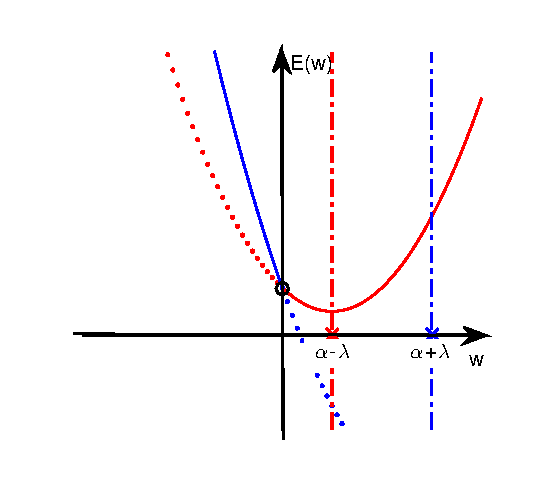
\includegraphics[width=1\textwidth]{figure/4-3(1)new.eps}
     \caption{$\alpha_i>\lambda$}
     \label{fig1}
\end{minipage}
\hfill
\begin{minipage}[t]{0.3\linewidth}
     \centering
     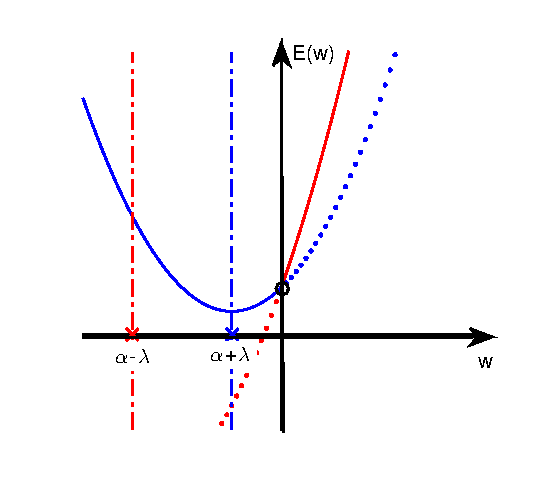
\includegraphics[width=1\textwidth]{figure/4-3(2)new.eps} 
     \caption{$\alpha_i<-\lambda$}\label{fig2}
\end{minipage}
\hfill
\begin{minipage}[t]{0.3\linewidth}
     \centering
     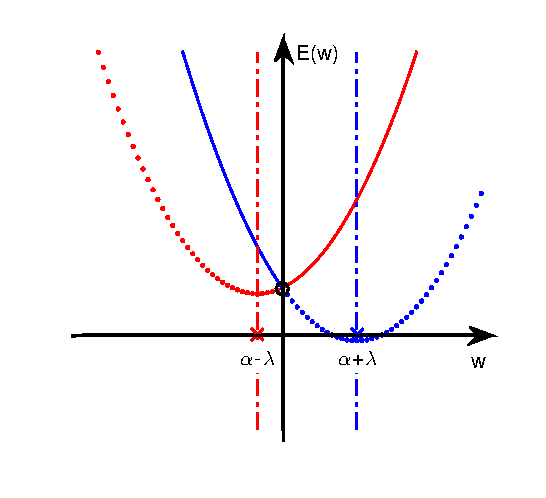
\includegraphics[width=1\textwidth]{figure/4-3(3)new.eps} 
     \caption{$-\lambda\leq\alpha_i\leq\lambda$}\label{fig3}
\end{minipage}
\end{figure}
\begin{itemize}
\item[(i).] $\alpha_i>\lambda$. As shown in Fig.(\ref{fig1}), the solid lines are plots of $E_{LASSO}(\bm{w})$, composed of two quadratic segments. The two symmetric axises are at the positive side of $w$ axis, since $\alpha_i+\lambda>\alpha_i-\lambda>0$. Thus, the optimal $\hat{w}_i^*=\alpha_i-\lambda$.
\item[(ii).] $\alpha_i<-\lambda$. Similarly, as shown in Fig.(\ref{fig2}), both symmetric axises are at the negative side of $w$ axis. The optimal $\hat{w}_i^*=\alpha_i+\lambda$.
\item[(iii).] $-\lambda\leq\alpha_i\leq\lambda$. As shown in Fig.(\ref{fig3}), since $\alpha_i-\lambda<0<\alpha_i+\lambda$. The solid line shows that $E_{LASSO}(w)$ is decreasing when $w_i<0$ and increasing when $w_i>0$. Therefore, the optimal $\hat{w}_i^*=0$.
\end{itemize}
Thus, the optimal $\bm{\hat{w}_{LASSO}^*}$ could be give as ${(\bm{\hat{w}}_{LASSO}^*)_i}=\left\{ \begin{array}{ll} (\bm{X}^T\bm{y})_i-\lambda, & (\bm{X}^T\bm{y})_i>\lambda, \\ (\bm{X}^T\bm{y})_i+\lambda, & (\bm{X}^T\bm{y})_i<-\lambda, \\ 0, & \text{otherwise}. \end{array}\right.$, in which $(\cdot)_i$ indicates the $i$th dimension.

\item[(4).] Error measurement $E_{\ell_0}(\bm{w})=\frac{1}{2}\lVert \mathbf{y} - \mathbf X \mathbf{w} \rVert_2^2 +\lambda\sum_{i=1}^d \mathbb{I}[w_i \neq 0]$. In this case, consider different dimensions separately, since
\begin{eqnarray}\label{lastref}
E_{\ell_0}(\bm{w})&=&\frac{1}{2}(\bm{w}^T\bm{w}-2\bm{y}^T\bm{Xw}+\bm{y}^T\bm{y})+ \lambda\sum_{i=1}^d \mathbb{I}[w_i \neq 0]\nonumber\\
&=&\sum_{i=1}^d\left(\frac{1}{2}w_i^2-\alpha_iw_i+\lambda\mathbb{I}[w_i \neq 0]\right)+C,
\end{eqnarray}
where $\alpha_i=(\bm{X}^T\bm{y})_i$ denotes the $i$th dimension in $\bm{X}^T\bm{y}$, and $C=\frac{1}{2}\bm{y}^T\bm{y}$ is a constant. Because all dimensional components in Eq.(\ref{lastref}) are independent, the optimization problem is equivalent to minimize each component. Consider the following cases:
\begin{itemize}
\item[(i).] $w_i\neq 0$. We have $\hat{w}_i^*=\mathop{\arg\min}_{w_i}\frac{1}{2}w_i^2-\alpha_iw_i +\lambda=\alpha_i$, with minimal value $\lambda-\frac{1}{2}\alpha_i^2$.
\item[(ii).] $w_i= 0$. The resulting component $\frac{1}{2}w_i^2-\alpha_iw_i=0$.
\end{itemize}
Thus, the optimal parameter would be determined by $\hat{w}_i^*=\left\{ \begin{array}{ll}\alpha_i, & \lambda-\frac{1}{2}\alpha_i^2<0, \\0, & \lambda-\frac{1}{2}\alpha_i^2\geq 0.\end{array}\right.$, i.e. $(\bm{\hat{w}_{\ell_0}^*})_i =\left\{ \begin{array}{ll}(\bm{X}^T\bm{y})_i & \frac{1}{2}(\bm{X}^T\bm{y})_i^2>\lambda, \\0, & \frac{1}{2}(\bm{X}^T\bm{y})_i^2\leq\lambda.\end{array}\right.$, in which $(\cdot)_i$ indicates the $i$th dimension.

In this problem, we can access the closed form solution thanks to the orthogonality of $X$, i.e. $\bm{X}^T\bm{X}=\bm{I}$. Without such restriction, the problem could be hard because
\begin{itemize}
\item the $\bm{w}^T\bm{X}^T\bm{Xw}$ term makes different dimensions correlate, so the analysis mentioned above may not apply;
\item the $\lambda \lVert \mathbf{w}\rVert_0$ term leads the point 0 to be a highly non-analytical(non-differentiable) case, making all gradient-based methods(gradient descent, Newton's method, etc.) hard to work; the function is even not continuous at the point 0, which is disastrous for all local search-based algorithms(coordinate descent, etc.);
\item the error function is non-convex according to the inspection of Jensen Inequality\cite{ref: nonconvex}.
\end{itemize}
\end{solution}

\begin{thebibliography}{99}
\bibitem{ref: singular} Stack Overflow, \textit{Matlab: How to find out if a matrix is singular?}.\\ \url{http://stackoverflow.com/a/13146750}.
\bibitem{ref: nonconvex} Ayush Bhatnagar. \textit{Why is the 'L0' norm non-differentiable and non-convex?} (2016). \\ \url{https://www.quora.com/Why-is-the-L0-norm-non-differentiable-and-non-convex}.
\end{thebibliography}

\end{document}